\begin{figure}[h!]
	\centering
	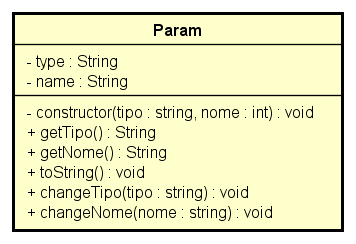
\includegraphics[scale=0.8]{res/sections/SpecificaFrontEnd/Services/Disegnetti/param.png}
	\caption{Diagramma della classe Param}
\end{figure}

\begin{itemize}
	\item \textbf{Descrizione:}\\
	
	\item \textbf{Utilizzo:}\\
	
	\item \textbf{Metodi:}
		\begin{itemize}
			\item \emph{-type: string}\\
    		Tipo del parametro
    		\item \emph{-name: string}\\
    		Nome del parametro
		\end{itemize}
	\item \textbf{Metodi:}
		\begin{itemize}
			\item \emph{-constructor(tipo: string, nome: string)}\\
    		Costruisce un nuovo parametro\\
    		\textbf{Parametri:}
    		\begin{itemize}
    			\item \emph{tipo: string}\\
    			Tipo del parametro
    			\item \emph{nome: string}\\
    			Nome del parametro
    		\end{itemize}
    		\item \emph{+getTipo()}\\
    		Ritorna il tipo del parametro
    		\item \emph{+getNome()}\\
    		Ritorna il nome del parametro
    		\item \emph{+toString()}\\
    		
    		\item \emph{+changeTipo(tipo: string)}\\
    		Modifica il tipo del parametro\\
    		\textbf{Parametri:}
    		\begin{itemize}
    			\item \emph{tipo: string}\\
    			Tipo del parametro
    		\end{itemize}
    		\item \emph{+changeNome(nome: string)}\\
    		Modifica il nome del parametro\\
    		\textbf{Parametri:}
    		\begin{itemize}
    			\item \emph{nome: string}\\
    			Nome del parametro
    		\end{itemize}
    	\end{itemize}
\end{itemize}